\documentclass{beamer}
\usepackage[utf8]{vietnam}
\mode<presentation> {
\usetheme{madrid}
%\setbeamertemplate{footline} % To remove the footer line in all slides uncomment this line
\setbeamertemplate{footline}[page number] % To replace the footer line in all slides with a simple slide count uncomment this line

\setbeamertemplate{navigation symbols}{} % To remove the navigation symbols from the bottom of all slides uncomment this line
}

\title{Tiny Shell}
\author{Giảng viên hướng dẫn: \textit{TS.} Phạm Đăng Hải\\
		Sinh viên:\\Hoàng Minh Tân\\Đặng Lâm San}
\institute{
Đại học bách Khoa Hà Nội
}
\date{\today}

\begin{document}
\begin{frame}
\titlepage
\end{frame}

%\begin{frame}
%\frametitle{Mục lục}
%\tableofcontents
%\end{frame}

%\begin{frame}
%\frametitle{Giới thiệu}
%
%\end{frame}

\begin{frame}
\frametitle{Các chức năng cơ bản}
Thao tác với shell bằng cú pháp : \textit{<command> -[option] [parameters]} (lệnh + tùy chọn + tham số).\pause
\begin{itemize}
\item Shell có một số lệnh cơ bản như: help, date, time, dir... cung cấp thông tin về shell, ngày tháng, thư mục shell đang trỏ tới ,...\pause
\item Shell có thể thao tác với tiến trình: tạo tiến trình dưới dạng \textit{foreground} hoặc \textit{background}, in ra danh sách tất cả tiến trình hoặc danh sách các tiến trình con của một tiến trình, hỗ trợ các thao tác quản lý 1 tiến trình như \textit{suspend, resume, kill}. Shell có thể nhận thao tác ngắt từ bàn phím.\pause
\item Thao tác với biến môi trường: in ra danh sách biến môi trường, thay đổi hoặc thêm mới biến môi trường.
\end{itemize}
\end{frame}

\begin{frame}
\frametitle{Các lệnh cơ bản}
Để thêm thông tin về các lệnh mà shell hỗ trợ, ta sẽ dùng lệnh \textit{help} hoặc \textit{help -[command]} để thêm thông tin về các tùy chọn mà  hỗ trợ.\\\pause
Một số lệnh cơ bản khác:\pause
\begin{itemize}
\item \textit{date, time}: xem thông tin về ngày và giờ .\pause
\item \textit{dir}: xem thông tin về các tập tin và thư mục con nằm trong thư mục shell đang trỏ tới.\pause
\item \textit{cd}: chuyển đường dẫn của thư mục shell đang làm việc tới một thư mục khác, ví dụ "cd C:/".\pause
\item \textit{exit}: thoát khỏi shell.
\end{itemize}
\end{frame}

\begin{frame}
\frametitle{Các lệnh cơ bản}
\begin{center}
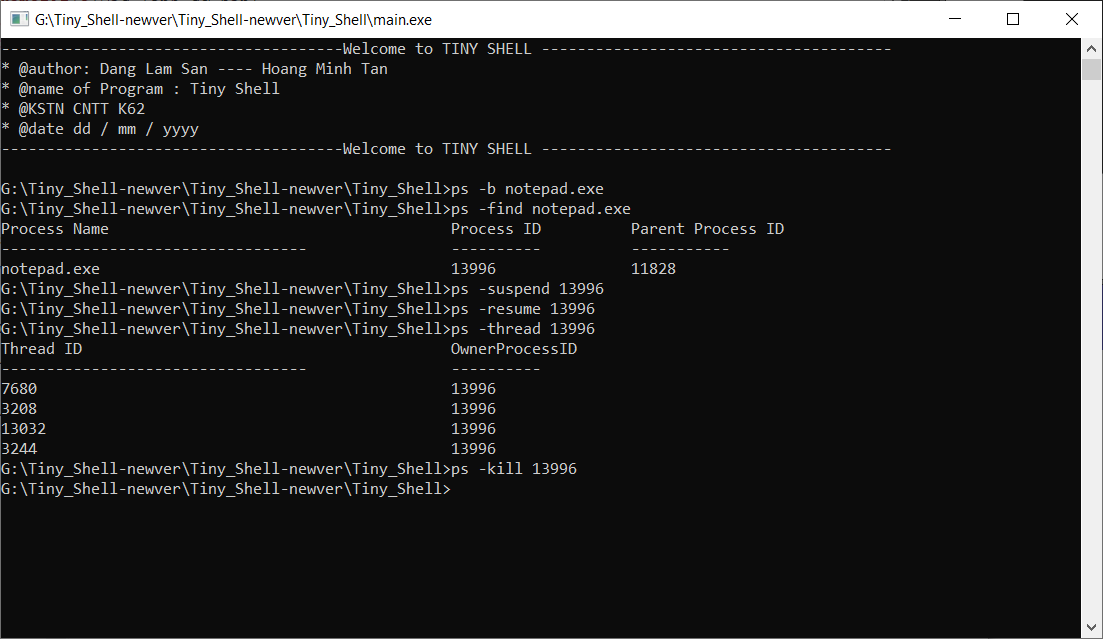
\includegraphics[scale=0.45]{process.png}
\end{center}
\end{frame}

\begin{frame}
\frametitle{Thao tác với tiến trình}
Shell cho phép người sử dụng làm việc với các tiến trình bằng lệnh \textit{ps} với các tùy chọn:\pause
\begin{itemize}
\item \textit{f, b}: khởi tạo một tiến trình dưới dạng foreground (f) hoặc background (b). Shell có thể nhận thao tác ngắt (CTRL+C) từ bàn phím để hủy bỏ tiến trình dưới dạng foreground.\pause
\item \textit{all}: xem thông tin của tất cả các tiến trình đang chạy.\pause
\item \textit{find}: lấy id của (các) tiến trình với tên cho trước.\pause
\item \textit{child}: xem thông tin các tiến trình con của tiến trình với cho trước.\pause
\item \textit{suspend, resume, kill}: tạm dừng, tiếp tục hoặc hủy bỏ một tiến trình với id cho trước.\pause
\item \textit{thread}: liệt kê tất cả các luồng của một tiến trình.
\end{itemize}
\end{frame}

\begin{frame}
\frametitle{Thao tác với tiến trình}
\begin{center}
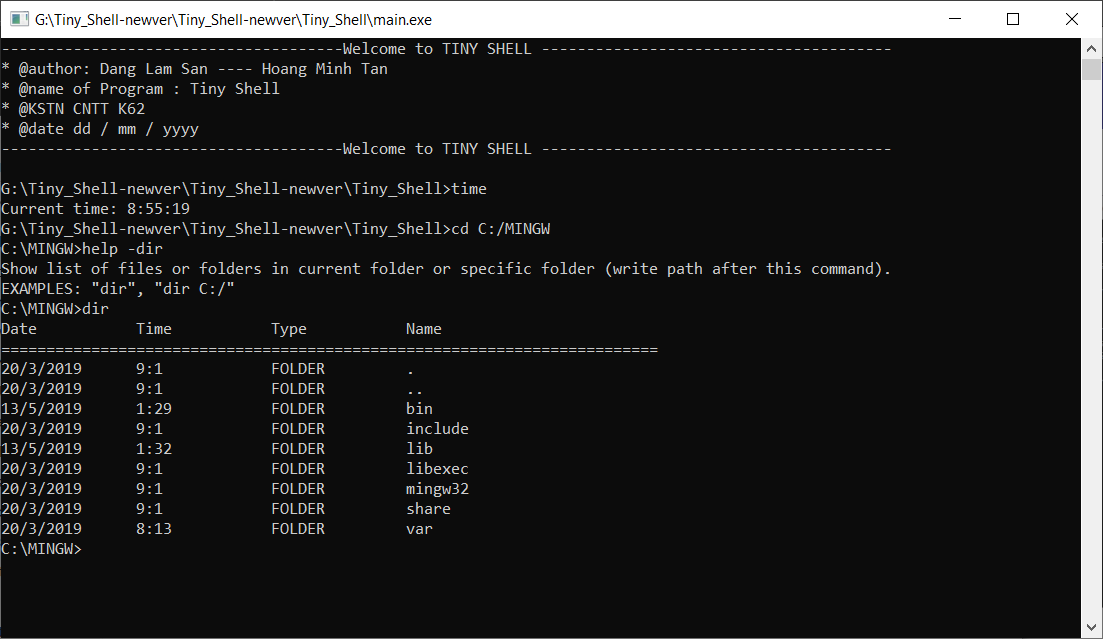
\includegraphics[scale=0.45]{basic.png}
\end{center}
\end{frame}

\begin{frame}
\frametitle{Thao tác với biến môi trường}
Shell cho phép làm việc với các biến môi trường thông qua lệnh \textit{enva}:\pause
\begin{itemize}
\item \textit{all}: xem tất cả các biến môi trường.\pause
\item \textit{get}: xem thông tin một biến môi trường.\pause
\item \textit{set}: tạo mới hoặc đặt lại một biến môi trường.\pause
\end{itemize}
\end{frame}

\begin{frame}
\frametitle{Thao tác với tiến trình}
\begin{center}
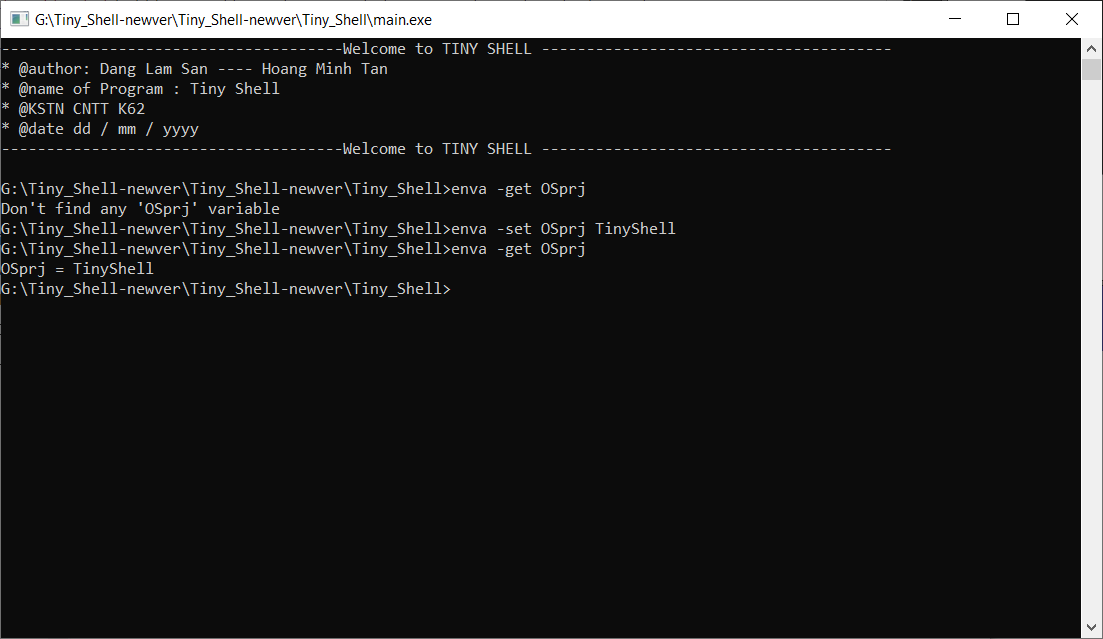
\includegraphics[scale=0.45]{environment.png}
\end{center}
\end{frame}

\begin{frame}
\frametitle{Kết luận}
\begin{center}
\begin{huge}
 Cảm ơn thầy và các bạn đã lắng nghe!
\end{huge}
\end{center}
\begin{center}
\begin{LARGE}
Q\&A
\end{LARGE}
\end{center}
\end{frame}

\end{document}